\section{Resultados y análisis}
\subsection{Equivalente electríco}

\begin{figure}[h]
    \centering
    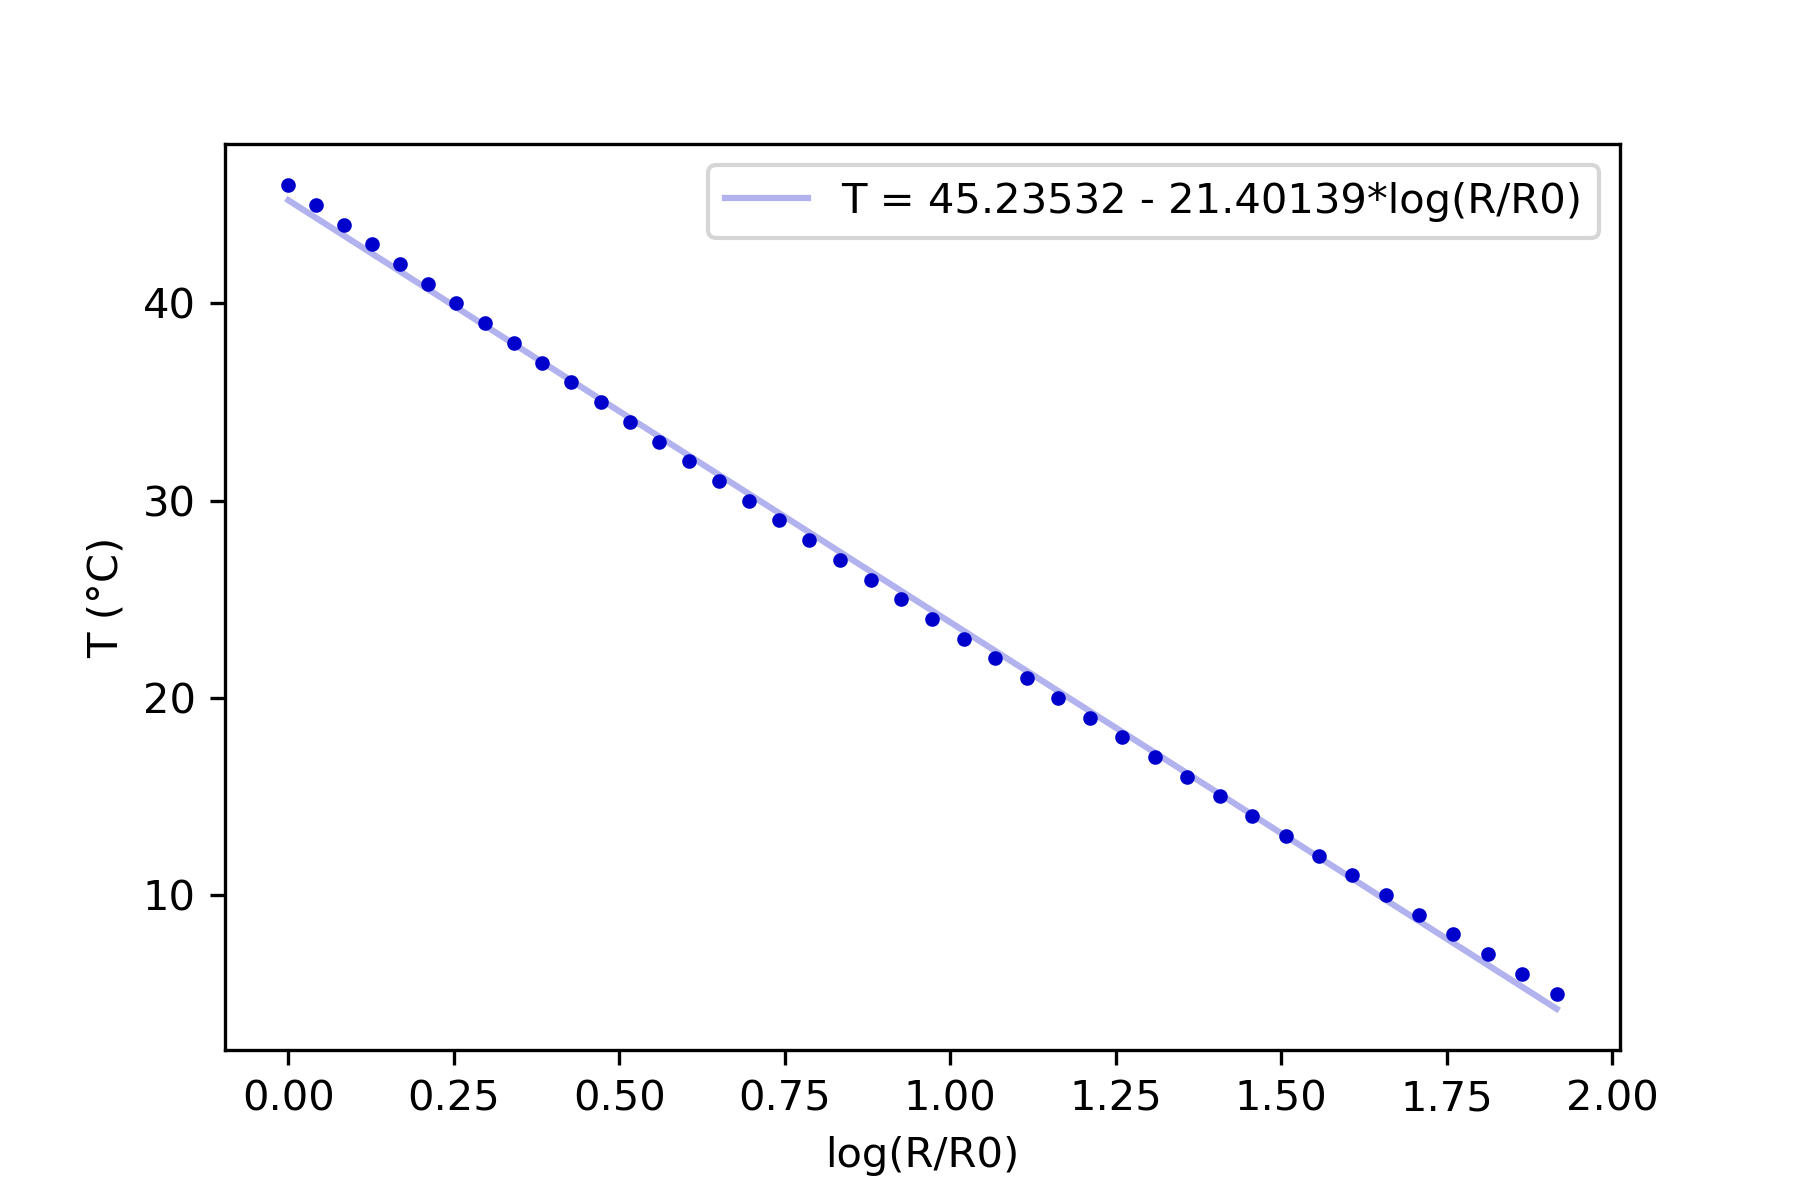
\includegraphics[width=0.35\linewidth]{img/termometric_curve.png}
    \caption{Curva termométrica del termistor usado.}
    \label{fig:termometric_curve}
\end{figure}

Usando los datos del fabricante del termopar, se obtiene la siguiente curva termométrica termistor es $T(R/R_0) = 45.2 - 21.4\ln(R/R_0)$ (ver figura \ref{fig:termometric_curve}). Con esta función, se transformaron los datos medidos de resistencia a valores de temperatura. Graficando temperatura contra tiempo se tiene lo mostrado en la figura \ref{fig:T_vs_t}; en la tabla \ref{tab:T_vs_t} se muestra el resumen de la linealización.

\begin{figure}[t]
    \centering
    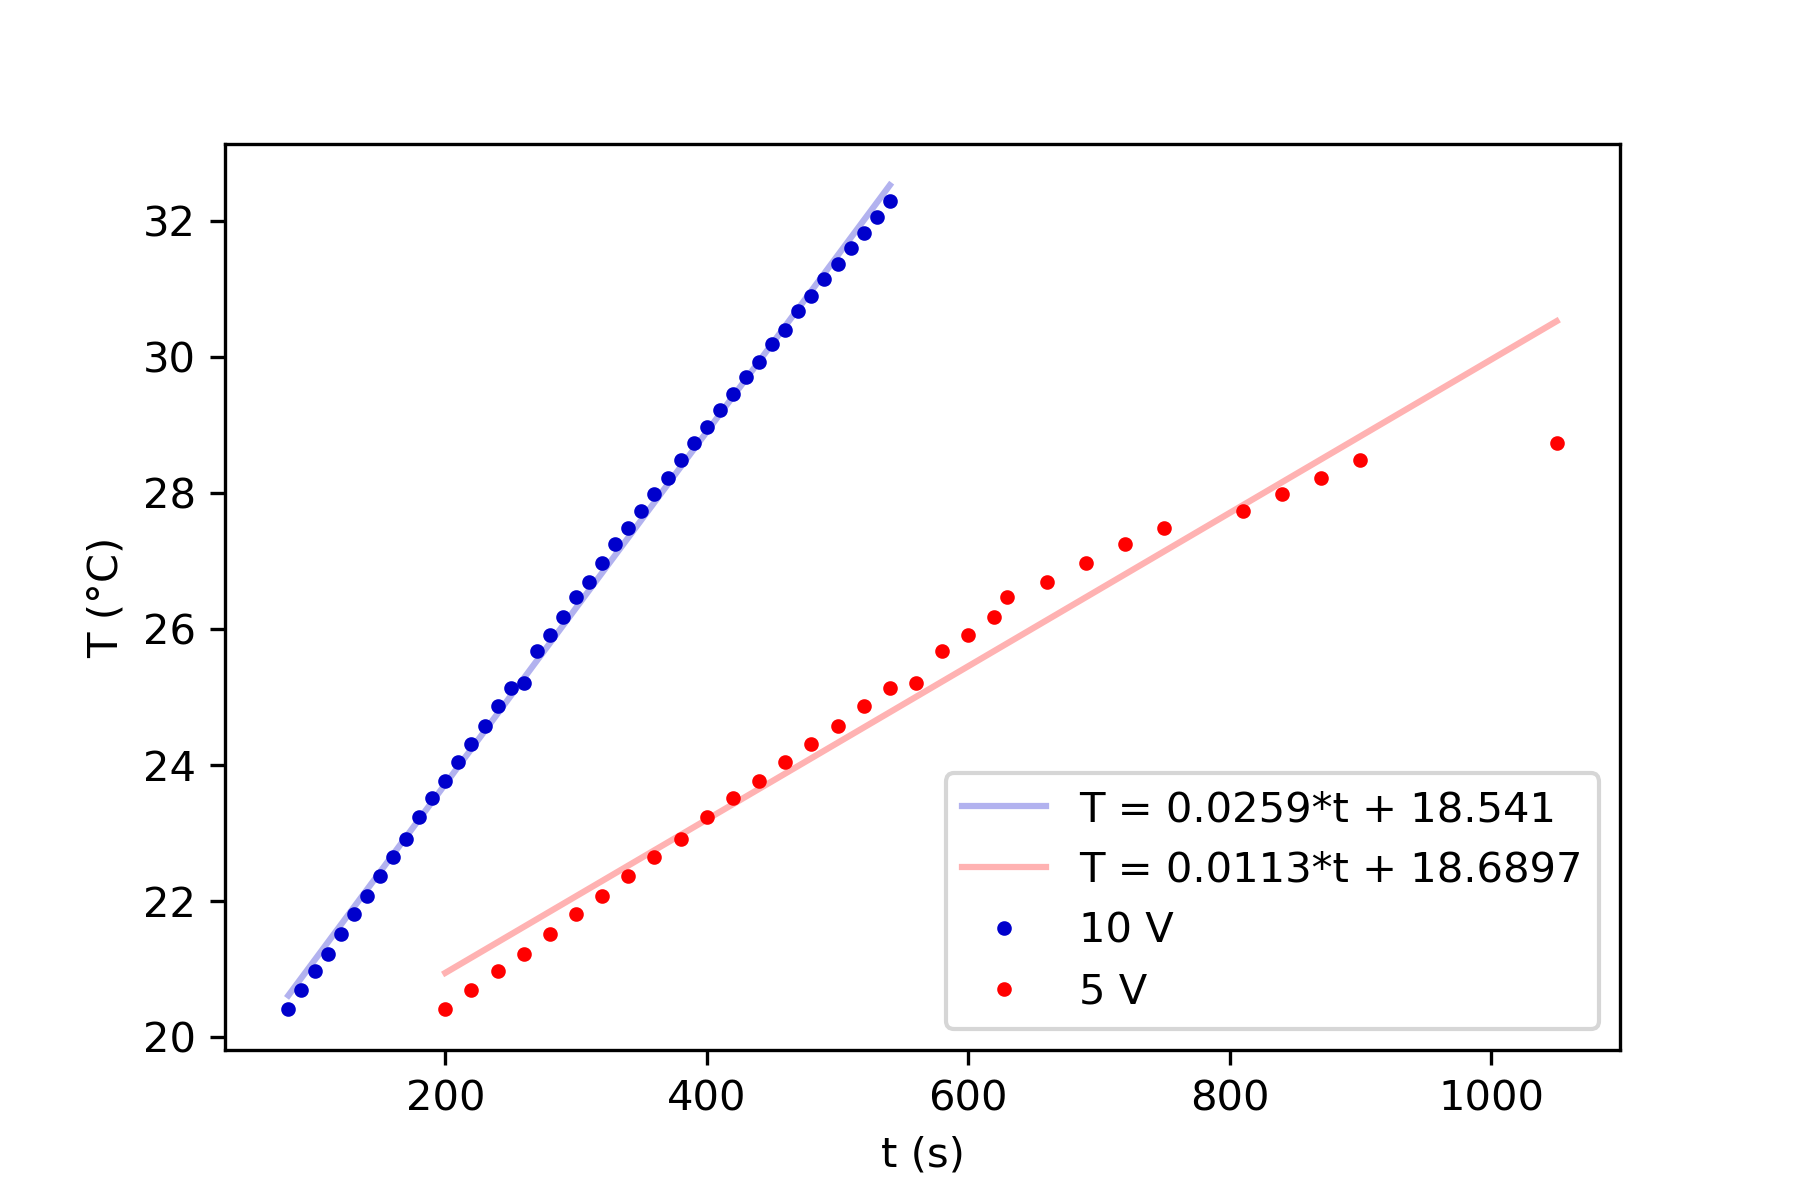
\includegraphics[width=0.6\linewidth]{img/T_vs_t.png}
    \caption{Temperatura contra tiempo del el agua dentro del calorímetro, para dos valores del potencial aplicado a la resistencia.}
    \label{fig:T_vs_t}
\end{figure}

\begin{table}[h]
    \centering
    \begin{tabular}{cccc}
        \toprule
        Toma & $\dot T$ & error & $R^2$ \\
        \midrule
        1 & $0.0113$ & $0.0008$ & $0.965 $\\
        2 & $0.0259$ & $0.0003$ & $0.999 $\\
        \bottomrule
    \end{tabular}
    \caption{valores para $\dot T = \Delta T/\Delta t$}    
    \label{tab:T_vs_t}    
\end{table}



\begin{table}[h]
    \centering
    \begin{tabular}{ccc}
        \toprule
        Toma & $J_{\text{elec}}$ & $\Delta J_{\text{elec}}$ \\
        \midrule
        1 & $1.323$& $0.014$\\
        2 & $0.1536$ & $0.0001$ \\
        \bottomrule
    \end{tabular}
    \label{tab:elec_equiv}        
\end{table}

\subsection{Equivalente mecánico}

\begin{figure}[H]
    \centering
    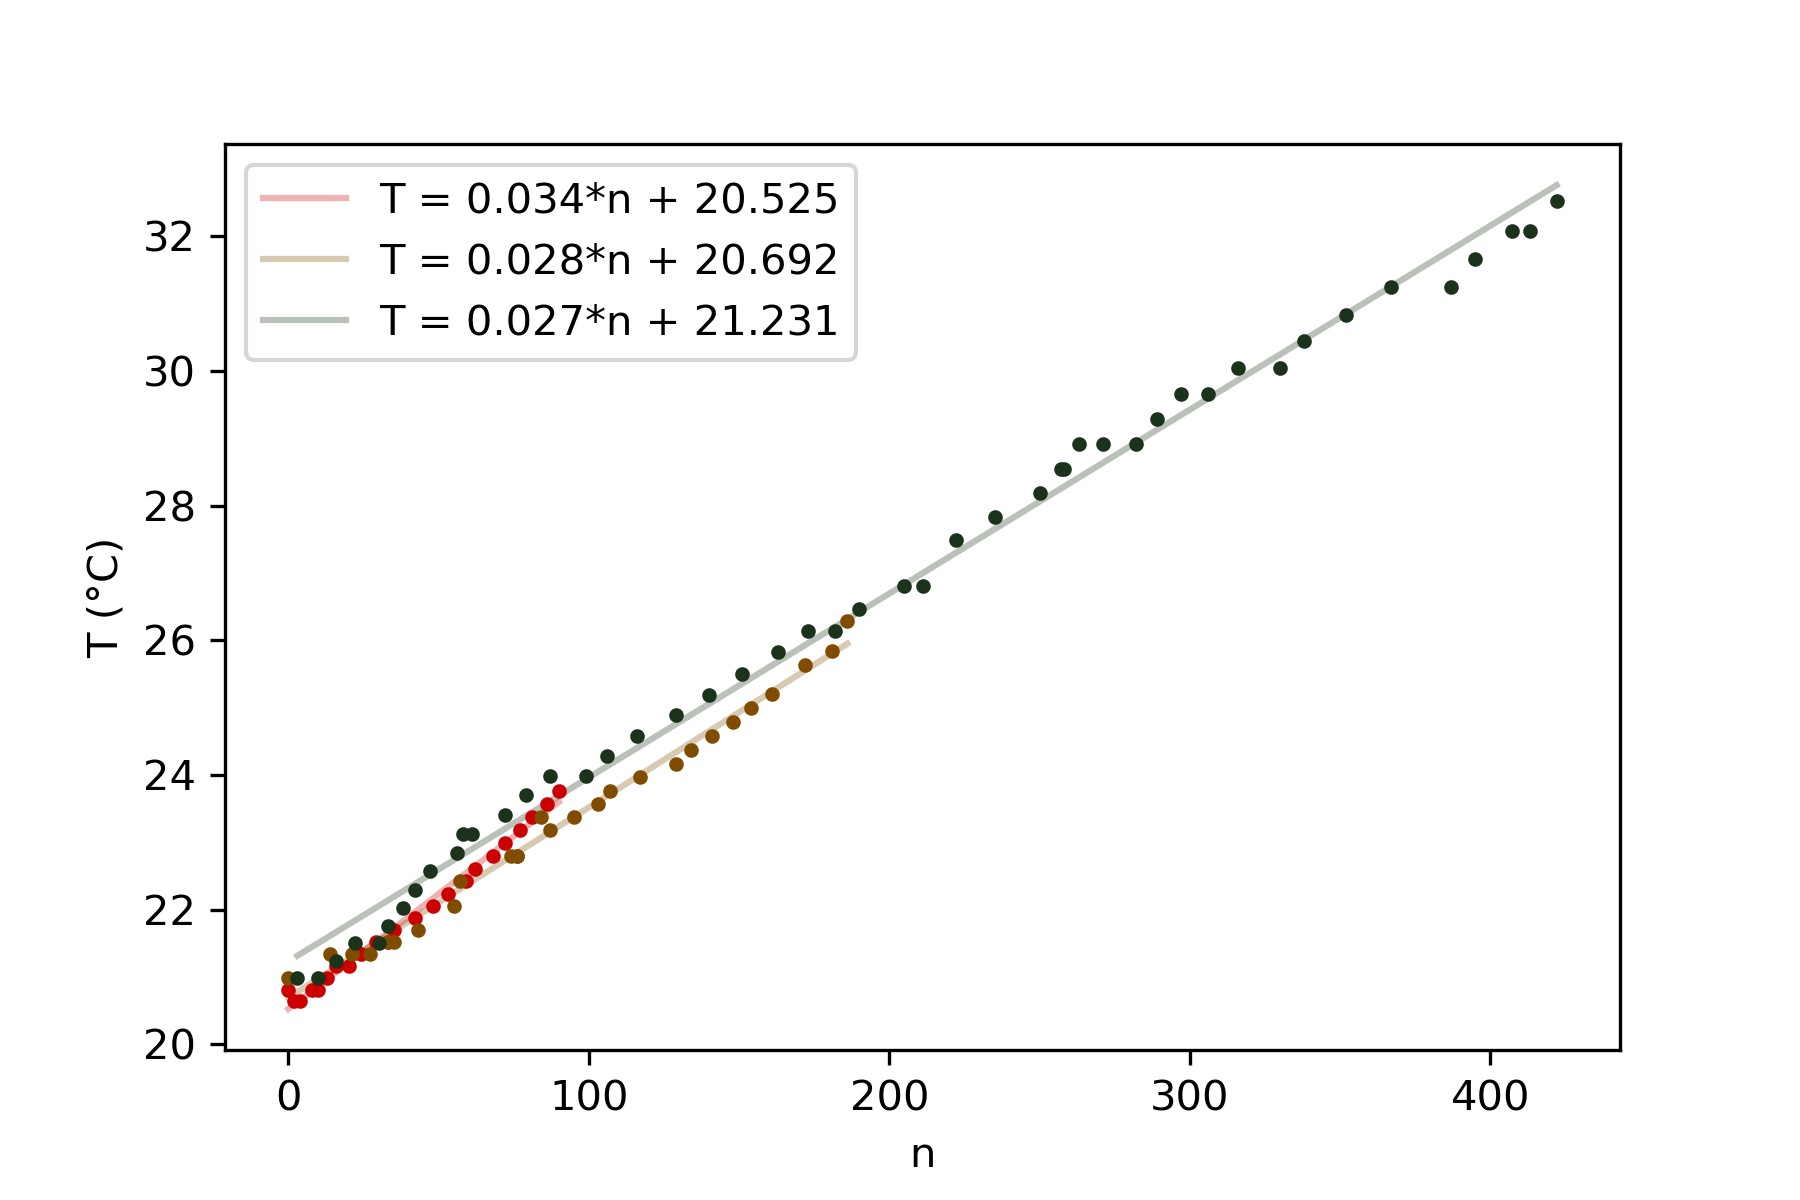
\includegraphics[width = .8\linewidth]{img/T_vs_N.png}
    \captionsetup{width=.6\linewidth}
    \caption[Temperatura como función del número de vueltas]{asdasd}
    \label{fig:T_vs_N_mec}
\end{figure}

\begin{table}[h]
    \centering\begin{tabular}{cccc}
        \toprule
        Toma & $\Delta T/\Delta n$ & error & $R^2$ \\
        \midrule
        1 & $0.0342$ & $0.0015$ & $0.9905$ \\
        2 & $0.0283$ & $0.0011$ & $0.9905$ \\
        3 & $0.0273$ & $0.0006$ & $0.9943$ \\
        \bottomrule
        \end{tabular}
    \caption{Valores medidos para $\Delta T/\Delta n$}
    \label{tab:T_vs_N}
\end{table}

De aquí la pendiente media $\frac{\Delta T}{\Delta n} = (0.0318 \pm 0.0019) \si{\celsius}$. De aquí se tiene que, usando la ecuación \eqref{eq:mechanical_equivalent}, $J_{\text{elec}} = (3.023 \pm 0.009)\,\si{\joule\per\calorie}$

